\documentclass[a4paper]{article}
\usepackage[dutch]{babel}
%\usepackage{eurosym}
%\usepackage{hyperref}
%\usepackage{graphicx}
%\usepackage{amsmath}
%\usepackage{amssymb}
%\graphicspath{{./Images/}}
\usepackage{verslag}

\begin{document}

\section{Analyse oude systeem}
In dit hoofdstuk worden responsie en de mechanische aspecten van het huidige mechanisme afgeleid en behandeld. Aan het einde van dit hoofdstuk worden conclusies getrokken over de sterke en zwakke punten van het huidige systeem, dit zal worden meegenomen in de conceptfase.

\subsection{Algemene informatie} (misschien hoort dit meer in de inleiding en het stukje over shortening in concepten)
\begin{figure}[h]
\label{oude_systeem}
\centering
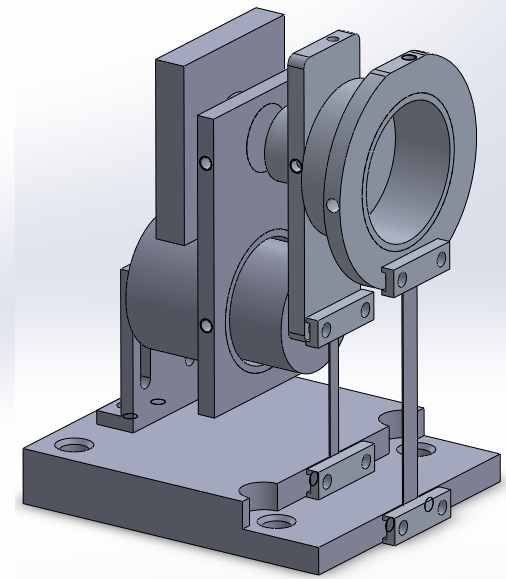
\includegraphics[width=0.5\textwidth]{SWmodel_oude_systeem.png}
\caption{3d model van het huidige systeem}
\end{figure}
\\
Zoals in figuur \ref{oude_systeem} te zien is, bestaat de huidige rechtgeleiding uit twee bladveren van verschillende lengte. Verder valt gelijk op te merken dat door het gebruik van twee bladveren het systeem overbepaald is. Ook is op te merken dat de bladeren worden ingeklemd met schroeven.

Bij het gebruiken van twee bladveren treedt er shortening op, dit wil zeggen dat het blok bij een uitwijking niet op gelijke hoogte blijft zitten. Er zijn twee bladveren met een verschillende lengte dus voor elke bladveer is de shortening berekende aan de hand van,
\begin{equation}
y=\frac{-0.6x^2}{l}
\end{equation}
Als maximale uitwijking van het systeem is 7.5mm genomen, volgens figuur \ref{Shortening} blijkt dat het shortening effect dan 1.3mm is. Echter is voor de exacte volging van de VCM, alleen een translatie in de x-richting gewenst. Door shortening vindt echter ook een kleine beweging in de y-richting plaats. Om deze beweging zoveel mogelijk te neutraliseren zou er een constructie moeten komen die shortening tegen gaat. 
\begin{figure}[h]
\label{Shortening}
\centering
\setlength\figureheight{5cm}
\setlength\figurewidth{0.9\textwidth}
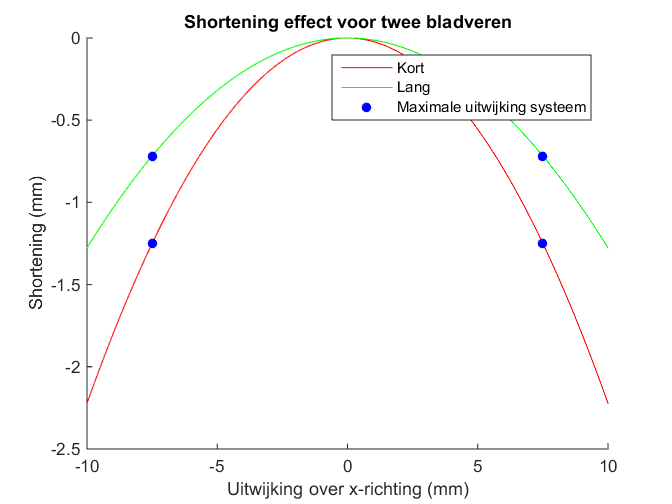
\includegraphics[width=0.75\textwidth]{Shortening.tikz}
\caption{Daling Blokje door Shortening}
\end{figure}


\clearpage


\subsection{Systeemresponsie}
Met behulp van een van de beschikbaar gestelde opstellingen (opstelling 12) is de stapresponsie (figuur \ref{opstelling_stapresp}) bepaald met behulp van een blokvormig signaal van amplitude 3 (figuur \ref{blokvormig}).
\begin{figure}[h]
\label{blokvormig}
  \centering
    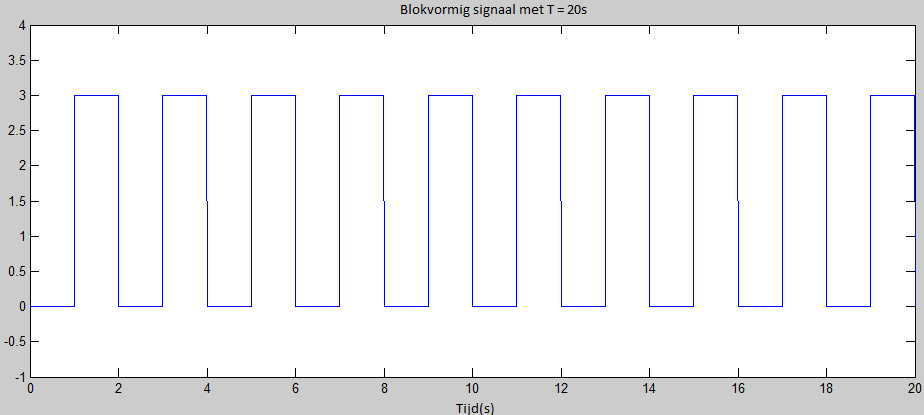
\includegraphics[width=0.55\textwidth]{Inputsignaal.png}
    \caption{Het gebruikte blokvormig signaal}
\end{figure}

\begin{figure}[h]
\label{opstelling_stapresp}
  \centering
    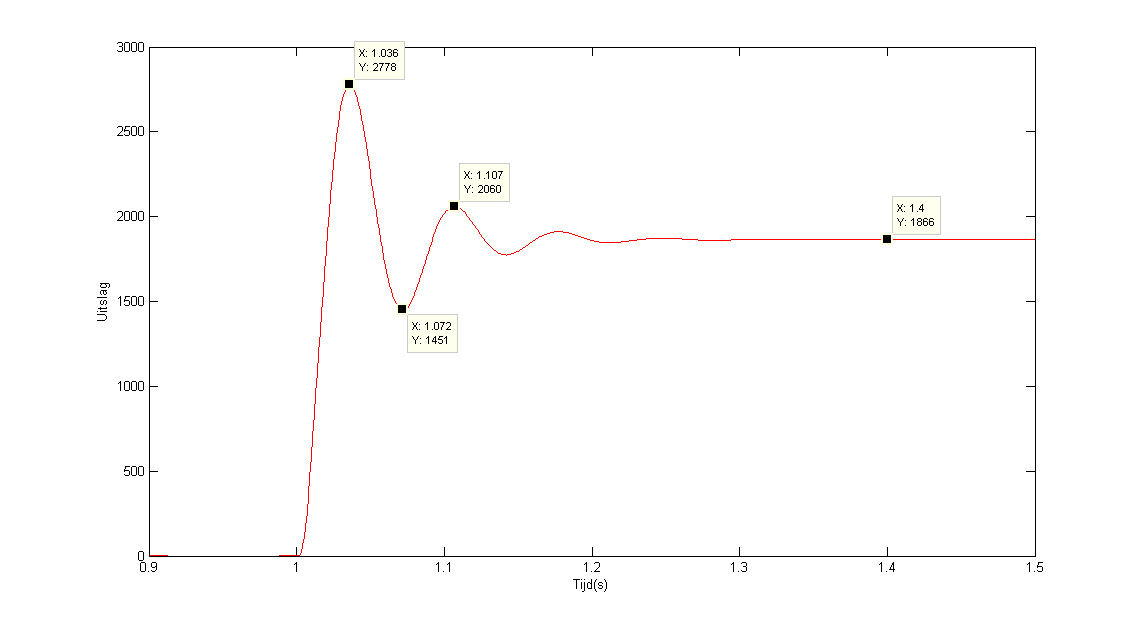
\includegraphics[width=0.95\textwidth]{Opstelling_12_stapresponsie.png}
    \caption{Representatieve stapresponsie met data-markers}
\end{figure}

Aangezien het huidige systeem gezien kan worden als een gedempt massa-veersysteem, kan de responsie van dit systeem vervolgens gemodeleerd worden met een tweede orde overdrachtsfunctie. 
\begin{equation}
G(s) = K * \frac{\omega_n^2}{s^2 + 2 \zeta \omega_n s + \omega_n^2}
\end{equation}
Met behulp van de overshoot en de peak-time die te bepalen zijn uit figuur \ref{opstelling_stapresp}) kunnen $\zeta$, $\omega_n$ en de versterking $K$ bepaalt worden.
\begin{equation}
\zeta = \frac{1}{\sqrt{1 + (\frac{\pi}{\ln(OS})^2}} \ \ \ with \ \ OS = \frac{x(t_p)}{x(\infty)} -1
\end{equation}
\begin{equation}
\omega_n = \frac{\pi}{t_p \sqrt{1 - \zeta^2}} \ \ derived \ from \ \ \omega_d = \frac{\pi}{t_p} \ \ and \ \ \omega_d = \omega_n \sqrt{1-\zeta^2}
\end{equation}
\begin{equation}
K = \frac{x_{response}(\infty)}{x_{signal}(\infty)}
\end{equation}
De waarden voor $K$, $\zeta$ en $\omega_n$ zijn dus gelijk aan: $ K = 622$, 
$\zeta = 0.223$ en $\omega_n = 89.5 \frac{rad}{s} = 14.2 \ Hz$.\\
De overdrachtsfunctie van dit systeem wordt dus gelijk aan:
\begin{equation}
G(s) = 622 * \frac{8013}{s^2 + 39.86 s + 8013}
\end{equation}
\begin{figure}[h]
\label{benadering_stapresp}
  \centering
    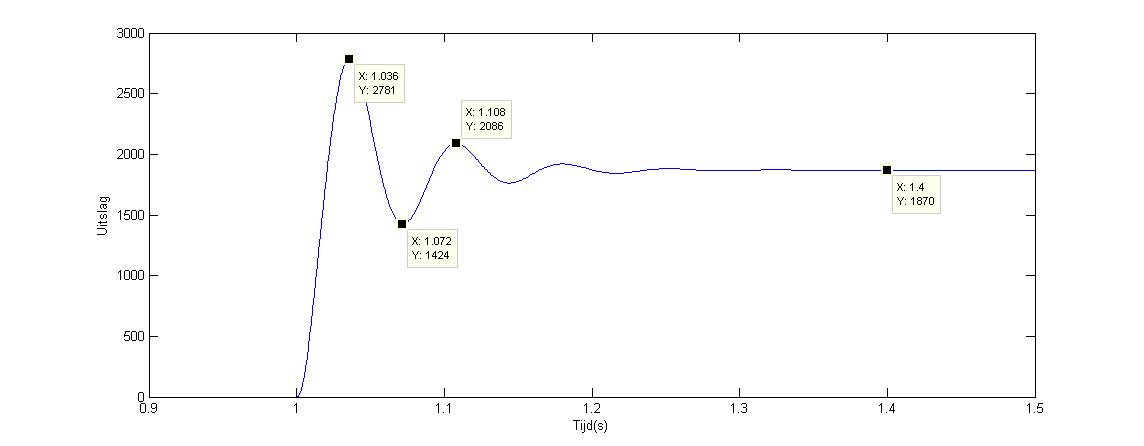
\includegraphics[width=0.95\textwidth]{overdrach_stap.png}
    \caption{gesimuleerde stapresponsie met data-markers}
\end{figure}
\\ \\
Als figuren \ref{opstelling_stapresp} en \ref{benadering_stapresp} met elkaar vergeleken worden word bevestigd dat de berekende overdrachtsfunctie een goede benadering is van dit systeem.


\subsection{Mechanische constanten}
Om het systeem later met de concepten te vergelijken, is het handig om de mechanische constanten van het systeem te bepalen. De mechanische constanten die bepaald kunnen worden zijn de massa van het (bewegende) systeem, de dempingsconstante en de veerconstante.  \\ 

Omdat de massa en de veerconstande gerelateerd zijn aan de eigenfrequentie van het systeem, en de veerconstante slechts afhangt van de bladveergeometrie, is het met behulp van formule \ref{Eigenfrequentie1} mogelijk om de massa van het systeem te bepalen. 

\begin{equation}
\omega_n=\sqrt{\frac{k_{eq}}{m}}, \ \ \ \omega_n= 89.5 \frac{rad}{s}
\label{Eigenfrequentie1}
\end{equation}

Om de equivalente veerconstante van het systeem te bepalen, wordt gebruik gemaakt van formule \ref{Veerstijfheid} en tabel \ref{bladveermaten}. Dit geeft $k_1=864$$N/m$, $k_2=256$$N/m$, invullen in formule \ref{Eigenfrequentie1} geeft een massa van 140g.
\\
\begin{table}[h]
\label{bladveermaten}
\begin{tabular}{lll}
                              & \textit{\textbf{1}} & \textit{\textbf{2}} \\
\textit{\textbf{Lengte (l)}}  & 27                  & 48                  \\
\textit{\textbf{Breedte (h)}} & 3                   & 5                   \\
\textit{\textbf{Dikte (t)}}   & 0.3                 & 0.3                
\end{tabular}
\caption{Afmetingen van de bladveren in het oude systeem in mm}
\end{table}
 
\begin{equation}
k=\frac{Eht^3}{l^3}, \ \ \ E = 210*10^9 pa \ \ \ k_{eq}=k_1+k_2
\label{Veerstijfheid} 
\end{equation} 

 De dempingsconstante van dit systeem kan  berekend worden aan de hand van\ref{SPACARtut}:
\begin{equation}
2\zeta\omega_n=\frac{d}{m} \ \ met: \ \zeta = 0.223 \ \ \omega_n = 89.5 \frac{rad}{s} \ \ m = 0.14 kg
\end{equation} 
Dit geeft een totale dempingscoefficient in dit systeem van 5.6$Ns/m$. Wat wel belangrijk is, is dat het grootste deel van de dempingcoefficent word geleverd  door de VCM, en dat de bijdrage van de bladveren te verwaarlozen is.\\

\subsection{Eigenfrequenties}
Een van de belangrijkere eigenschappen van een ontwerp zijn de eigenfrequenties van het systeem. Het is wenselijk om de 1ste eigenfrequentie (van de ontworpen beweging) zo laag mogelijk te houden, terwijl de hogere eigenfrequenties (van de niet ontworpen bewegingen) zo hoog mogelijk gemaakt moeten worden om ongewenste bewegingen te onderdrukken. Het huidige systeem is in Spacar gemodeleerd, en in figuren ()etc zijn de berekende eigenfrequenties te zien. Te zien valt dat de eerste eigenfrequentie redelijk overeenkomt met de eerder berekende, terwijl de hogere eigenfrequenties op iets respectievelijk iets liggen.
\subsection{Conclusies en aanbevelingen}
Een van de nadelen van het oude systeem is al eerder behandeld namelijk dat door het gebruik van twee bladveren het systeem overbepaald is wat zorgt voor ongewenste spanningen in de bladverenveren. \\ Tijdens experimenten met de beschikbaar gestelde opstellingen zijn verder nog twee problemen duidelijk geworden. 
Ten eerste dat het systeem door het onwerp van de inklemming zeer snel klem kan komen te zitten door het draaien in de inklemming van de bladveren. 
En ten tweede dat het systeem zeer gevoelig is voor krachten van buitenaf (dit viel te zien in pieken als de opstellingstafel werd geraakt).  Dit kan gedeeltelijk opgevangen worden door de eigenfrequentie van het systeen te verhogen, hierdoor zal een invloed van buitenaf minder invloed hebben op de uitslag van het systeem. \\


\end{document}
